%--------------------
% document principal
%--------------------
% cal compilar amb `pdflatex -shell-escape main.tex`
% makeglossaries main
%--------------------
\documentclass[paper=a4,parskip=half,
twoside,fontsize=11pt,BCOR12mm,
%oneside,fontsize=11pt, %%format web
% twoside,openany,fontsize=10pt,DIV = 10,BCOR12mm, %%format en paper
]{scrbook}
%%%%BCOR12mm  factor de correcció per enquadernació
%%%%BCOR??mm  factor de correcció per enquadernació amb espiral -0.5mm??
%\usepackage[T1]{fontenc}
%------------- capçalera ----------------------
\input{capçalera.default}
\bibliography{bibliografia}
%\ExecuteBibliographyOptions{annotation=true,backref=true}
%backref=true, urldate=long, abbreviate=false,%%format web 
%---------- Mode esborrany --------------------
%\includeonly
%{model}
\usepackage[catalan]{todonotes} %%ús: \todo{text} \missingfigure{text}
\usepackage{fancyhdr}\pagestyle{fancyplain}\rhead{\fancyplain{--- esborrany \today\ ---}{\color{gray}{\today}}}\renewcommand{\headrulewidth}{0pt}
%\usepackage[showframe]{geometry}%page margins
%----------------------------------------------
%\usetikzlibrary{shapes,arrows,positioning}
%\usetikzlibrary{calc}
%------------- format -------------------------
%%ús coma decimal sense espais:  2{,}5
%per tal que trenqui la coma en math inline mode 
%http://tex.stackexchange.com/questions/19094/allowing-line-break-at-in-inline-math-mode-breaks-citations/
\AtBeginDocument{%
  \mathchardef\mathcomma\mathcode`\,
  \mathcode`\,="8000 
}
{\catcode`,=\active
  \gdef,{\mathcomma\discretionary{}{}{}}
}
%teoremes
\theoremstyle{plain}
\newtheorem{definition}{Definició}
\theoremstyle{definition}
\newtheorem{example}{Exemple}
\def\figureautorefname{figura} %ús: \autoref{}
\def\tableautorefname{taula} %ús: \autoref{}
\def\definitionautorefname{definició} %ús: \autoref{}
\def\exampleautorefname{exemple} %ús: \autoref{}
\def\sectionautorefname{secció} %ús: \autoref{}
\def\subsectionautorefname{apartat} %ús: \autoref{}
%numeracions d'equacions, definicions, etc.
\numberwithin{equation}{chapter}
\numberwithin{definition}{chapter}
\numberwithin{example}{chapter}



%glossaris
\usepackage[
          acronym,
          %%nonumberlist,
          %%toc,
          section,
          numberedsection=autolabel,
          sanitize=none, %pels accents en el vegeu
          ]{glossaries}
%\renewcommand*{\glspostdescription}{}%anul·la el punt final
\renewcommand*{\acronymname}{Sigles}%{Índex de sigles}??si té refs pàgines 
%Índex d'abreviacions?? si conté abreviatures o símbols
% \short<type>name,
\newglossary{notation}{not}{ntn}{Notació}
\newglossarystyle{estil-notation}{%
  \renewcommand{\glsgroupskip}{}% make nothing happen between groups
  \renewenvironment{theglossary}
  {\begin{longtable}{lll}
      % \caption{Notació dels SGSTM \label{tab:sgstm-simbols}}
      % \endfirsthead
      % \caption[]{Notació dels SGSTM (continuació)}
      % \endhead
          % \endfoot
          % \endlastfoot
    }{\end{longtable}}
  \renewcommand*{\glossarysubentryfield}[6]{%
    %\glstarget{##2}{##3}% the entry name
    \glstarget{##2}{\Glsentryname{##2}}% the entry name
    &
     %\space (##5)% the symbol in brackets
    \space ##4% the description
    &
    \space [##6]% the number list in square brackets
    \\
  }%
  \renewcommand*{\glossaryentryfield}[5]{%
    \\\pagebreak[3]\hline
    \glossarysubentryfield{##2}{##1}{##2}{##3}{##4}{##5}
    \hline
  }
}


\renewcommand{\seename}{vegeu}
\renewcommand{\entryname}{Notació}
\renewcommand{\descriptionname}{Descripció}

\makeglossaries


%\renewcommand{\glossarypreamble}{Text com a préambul}



%TERMES


%temps real
\newglossaryentry{TempsReal}{name={temps real}, description={(\emph{real time}), sistemes que han de respondre amb un temps determinat. A vegades també s'utilitza el terme com a adjectiu per a designar sincronització real amb el rellotge o per a indicar que l'usuari no percep retards. Allà on pugui causar confusió, utilitzarem sincronitzat o en línia (\emph{online}) per al segon significat.}
}





\newglossaryentry{SistemaGestioBaseDades}{name={sistema de gesti{ó} de base de dades}, description={(\emph{Data Base Management System})} }




%terme:SGBDR

\newglossaryentry{terme:SGBDR}{name={sistema de gestió de base de dades relacional}, description={(\emph{Relational Data Base Management System}). 
També anomenat 'object/relational' DBMS \parencite{date06}.
Totes les definicions són coherents amb \textcite{date:introduction} } }



%model, implementació
%Els SGBD es basen en teories matemàtiques que reben el nom de model de dades, un SGBD és una implementació d'un model de dades.
%Segons \citeauthor{date:introduction}, ``un model de dades és una definició abstracta, auto continguda i lògica dels objectes, de les operacions i  de la resta que conjuntament constitueixen la màquina abstracta amb la que els usuaris interactuen. Els objectes permeten modelar l'estructura de les dades. Les operacions permeten modelar el comportament''. Ara bé, \citeauthor{date:introduction} avisa que el concepte model de dades també s'usa per a definir una estructura persistent de dades concreta i per tant cal distingir adequadament la confusió entre els dos conceptes.
% Tal com fa Date, parlarem de model de dades en el primer sentit de màquina abstracta i a vegades ho abreviarem com a model.


%tipus,valor,variable,operador

\newglossaryentry{terme:SGBDR:domini}{see={terme:SGBDR},name={domini}, description = {(\emph{domain}), equivalent a tipus de dades.
Conjunt de valors. Cada domini té associat un conjunt d'operadors, en alguns casos fins i tot s'entén que el domini inclou els operadors (concepte de classe a orientació a objecte). Els tipus tenen una representació (estructura) o més d'una, és a dir els seus valors poden estar denotats per més d'un literal} }
\newglossaryentry{terme:SGBDR:tipus}{see={terme:SGBDR:domini}, name={tipus de dades}, description = {(\emph{data type}), a vegades solament 'tipus' (\emph{type}) o bé 'tipus de dades abstracte' (\emph{abstract data type}). Segons \textcite{date:introduction} en el context de model tots els tipus de dades han de ser abstractes} }

\newglossaryentry{terme:SGBDR:escalar}{parent={terme:SGBDR:domini}, name={escalar}, description = {Un tipus és escalar (\emph{scalar}) quan no té components visibles a l'usuari i és no escalar (\emph{nonscalar}) en cas contrari; no obstant, tant els escalars com els no escalars tenen representació, la qual pot contenir components} }


\newglossaryentry{terme:SGBDR:valor}{see={terme:SGBDR},name={valor}, description = {(\emph{value}), equivalent a objecte i instància.
'Constant individual' que és d'un tipus de dades. A vegades s'utilitza 'constant' per designar una  variable que mai canvia de valor, però aquest no és el cas d'aquesta definició} }
\newglossaryentry{terme:SGBDR:objecte}{see={terme:SGBDR:valor}, name={objecte}, description = {(\emph{object})} }
\newglossaryentry{terme:SGBDR:instancia}{see={terme:SGBDR:valor}, name={instància}, description = {(\emph{instance})} }

\newglossaryentry{terme:SGBDR:literal}{see={terme:SGBDR},name={literal}, description = {(\emph{literal}).
Símbol que denota un valor. Un valor pot estar denotat per més d'un literal. Segons aquesta definició literal no és equivalent a valor} }


\newglossaryentry{terme:SGBDR:variable}{see={terme:SGBDR},name={variable}, description = {(\emph{variable}).
Contenidor d'una aparició d'un valor. El valor que conté la variable pot ser canviat mitjançant l'operador d'assignació. En canvi els valors, per si mateixos, no poden ser actualitzats} } %A l'esquerra de l'operador d'assignació sempre hi ha variables, tot i que s'admeten simplificacions mitjançant expressions que són pseudovariables (p.ex. s[1] := 3 és equivalent a s := [s[0],3,s[2],..]).
%Les variables tenen adreces (\emph{addresses}) i per tant es pot apuntar (\emph{point to}) a les variables mitjançant els operadors de referència (\emph{referencing}), el qual retorna l'adreça d'una variable, i de desreferència (\emph{dereferencing}), el qual retorna la variable a partir de l'adreça. Els valors adreces pertanyen al tipus apuntador, però el model relacional prohibeix els valors de tipus apuntador i per tant no té REF ni DEREF; les relvar s'identifiquen pel seu nom i no cal que tinguin adreça. (Compte que en orientació a objectes una variable és el contenidor d'un valor que és un ID d'objecte, és a dir és el contenidor d'una referència).



%relació
\newglossaryentry{terme:SGBDR:relacio}{%
  see={terme:SGBDR},%
  name={relació},%
  plural={relacions},%
  sort={relacio},%
  description = {(\emph{relation}). Pot referir-se tant a tipus,
    valor, literal o variable relació. És l'objecte principal d'estudi
    en els SGBDR i de manera popular s'anomena taula. \emph{Nota}:
    hi ha certes diferències lògiques entre les relacions del model
    relacional i les relacions tal com es defineixen en matemàtiques.
  }%
}










%terme:tipus

% %reals projectius
% \newglossaryentry{terme:tipus:real-projectiu}{%
%   see={terme:SGBDR:tipus},%
%   name={real projectiu},%
%   plural={reals projectius},%
%   symbol={\ensuremath{\bar\mathbb{R}}},%
%   description = {(\emph{projective extended real
%       numbers}). 
% %$\bar\mathbb{R}\in\mathbb{R}\cup$
% %\{-\infty,+\infty\}$.
%   }%
% }





% [date2005]
% The original version of the model also omitted a few things I now consider vital. For example, it excluded any
% mention—at least, any explicit mention—of all of the following: predicates, constraints (other than candidate
% and foreign key constraints), relation variables, relational comparisons, relation type inference and associated
% features, certain algebraic operators (especially rename, extend, summarize, semijoin, and semidifference),
% and the important relations TABLE_DUM and TABLE_DEE.




%pendent: falta posar el name

% \newglossaryentry{SGBD-model}{ description = {Un model és}, name={Model de SGBD} }



% \newglossaryentry{SBDR-cap}{ description = {La capçalera d'un SGBDR}, name={Capçalera}, parent={SGBD-model} }



% \newglossaryentry{heading}{ description = {Equivalent to intension and relation schema} }
% \newglossaryentry{intension}{ description = {}, see=heading }
% \newglossaryentry{relation schema}{ description = {}, see=heading }

% \newglossaryentry{body}{ description = {Equivalent to extension} }
% \newglossaryentry{extension}{ description = {buit}, see=body}


% \newglossaryentry{DBMS data model}{ description = {A data model (first sense) is an abstract, self-contained, logical definition of the
% objects, operators, and so forth, that together constitute the abstract machine with which
% users interact. The objects allow us to model the structure of data. The operators allow us
% to model its behavior.\cite{date}. Sometimes it is referred as architecture.
% } }

% \newglossaryentry{data model}{ description = { A data model (second sense) is a model of the persistent data of some particular
% enterprise. [date06]. }}


% \newglossaryentry{DBMS implementation}{ description = {An implementation of a given data model is a physical realization on a real
% machine of the components of the abstract machine that together constitute that model.\cite{date}} }


% \newglossaryentry{data independence}{ description = {model and implementation kept separated}}




% \newglossaryentry{relationships}{
% description={relationships are semantic. relationships are entities.}}








%%% Local Variables: 
%%% mode: latex
%%% TeX-master: "../main"
%%% End: 

\loadglsentries{vocabulari/abreviacions.tex}
\loadglsentries[notation]{vocabulari/notacio.tex}
\newcommand{\glssymboldef}{\glssymbol[format=hyperbf,counter=definition]}
\newcommand{\glsdispdef}{\glsdisp[format=hyperbf,counter=definition]}
\newcommand{\hyperbfsec}[1]{\textbf{\S\hypersf{#1}}}
\newcommand{\hyperbfex}[1]{\textbf{ex.\hypersf{#1}}}
\newcommand{\glsaddsec}{\glsadd[format=hyperbfsec,counter=subsection]}
\newcommand{\glsdispsec}{\glsdisp[format=hyperbfsec,counter=subsection]}
\newcommand{\glssymbolsec}{\glssymbol[format=hyperbfsec,counter=subsection]}
\newcommand{\glssymbolex}{\glssymbol[format=hyperbfex,counter=example]}



%-------------- dades --------------------------
\hypersetup{
    pdftitle={Disseny i modelització d'un sistema de gestió multiresolució per a sèries temporals},
    pdfauthor={Aleix Llusà Serra},
    pdfcreator={DiPSE--UPC},
    pdfsubject={Tesi 2011--2014},
    pdfkeywords={sèries temporals; model de dades; sistemes de bases de dades; sistemes de monitoratge},
    pdflang={ca},
}

\title{Disseny i modelització d'un sistema de gestió multiresolució per a sèries temporals}
\author{Aleix Llusà Serra}
%----------------------------------------------


\begin{document}




\chapter{Esquemes de multiresolució}

\todo{}


Definim una funció de multiresolució com una consulta sobre una sèrie
temporal que ens retorna una nova sèrie temporal resultant
d'aplicar-li un esquema de multiresolució. 

Aquesta funció de multiresolució ens permetrà:

\begin{itemize}
\item Plantejar problemes on veiem la multiresolució com una consulta sobre una sèrie temporal
\item Oferir sistemes duals de \glspl{SGSTM} i \glspl{SGST} amb operacions
  de consulta multiresolució.
\item Estudiar implementacions per a la consulta de multiresolució, p.ex. para\l.lelisme. (vegeu secció implementació \todo{})
\item Estudiar la teoria de la informació per a l'esquema de multiresolució
\end{itemize}






\section{Funció de multiresolució}

En el model de \gls{SGSTM} hem definit un model de dades de \gls{SGBD}
per a gestionar sèries temporals multiresolució. Com a \gls{SGBD},
aquest model té una estructura i per tant emmagatzema informació d'una
sèrie temporal en una forma determinada: la de multiresolució.  La
definició com a \gls{SGBD} té com a objectius l'emmagatzematge
compacte de les dades i la selecció de la informació ja preparada per
a consultes posteriors. 

Així, aquest model té capacitats de computació
sincronitzada o en línia (\emph{online}) amb el temps i té
característiques dels sistemes que tracten fluxos de dades (\emph{data
  stream}); és a dir dades que s'estan adquirint contínuament i cal
anar computant al mateix temps que es van adquirint. Això no treu,
però, que de manera més simplificada també es pugui treballar amb un
\gls{SGSTM} en temps diferit (\emph{offline}), és a dir que
s'emmagatzemin les dades adquirides i en el moment que es vulgui
aplicar-hi la consolidació.




Això no obstant, podem simplificar el problema de càlcul de
multiresolució en temps diferit com una consulta en un \gls{SGST} de
transformació d'una sèrie temporal a una nova sèrie temporal.

És a dir, sigui $S$ una sèrie temporal, $M$ una sèrie temporal
multiresolució i $e = \{ (\delta_0,f_0,\tau_0,k_0), \ldots,
(\delta_d,f_d,\tau_d,k_d)\}$ els paràmetres de l'esquema de
multiresolució de $M$. Afegim totes les mesures de la sèrie temporal a
la multiresolució, $\forall m \in S:
M=\glssymbol{addM}(M,m)$\todo{matemàticament és correcte recursivitat
  M=f(M)?}, i la consolidem, $M=\glssymbol{consolidaM}(M')$ fins que
$M$ no sigui consolidable. Consultem la sèrie temporal multiresolució
amb les dues consultes bàsiques, les quals retornen sèries temporals,
$S'=\glssymbol{not:sgstm:serietotal}(M')$ i $S_{\delta
  f}'\glssymbol{not:sgstm:seriedisc}(M',\delta,f)$ on $\delta$ i $f$
són dos paràmetres de l'esquema de multiresolució de $M$ que van
associats amb els altres dos corresponents $\tau$ i $k$.



Plantegem les funcions de transformació de la sèrie temporal original
a les consultades. És a dir, les funcions que anomenem
$\glssymbol{not:sgstm:dmap}$ i $\glssymbol{not:sgstm:multiresolucio}$
i que ens permeten calcular:

\[
\glssymbol{not:sgstm:dmap}: S \times \delta \times f \times \tau \times k \longrightarrow
S'_{\delta f}
\]


\[
 \glssymbol{not:sgstm:multiresolucio}: S \times e  \longrightarrow S'
\]



Definim la consulta de selecció de disc dels \gls{SGSTM} a partir del
mapatge dels \gls{SGST} de manera que, en computació per temps
diferit, són equivalents
\[
\glssymbol{not:sgstm:seriedisc}(M',\delta,f) \equiv
\glssymboldef{not:sgstm:dmap}(S,\delta,f,\tau,k)
\]


\begin{definition}[mapa de \glssymbol{not:sgstm:seriedisc}]
  Sigui $S$ una sèrie temporal, $M$ una sèrie temporal multiresolució
  amb esquema $e$ i $(\delta,f,\tau,k)\in e$ els paràmetres de
  multiresolució d'una subsèrie resolució. L'expressió de
  $\glssymbol{not:sgstm:seriedisc}(M,\delta,f)$ com a mapa d'una sèrie
  temporal és $\glssymboldef{not:sgstm:dmap}(S,\delta,f,\tau,k)=
  \glssymbol{not:sgst:map}(S_I,\glssymbol{not:sgst:fmap})$ on
  \[
  \glssymbol{not:sgst:fmap}: m_i\mapsto f(S, [T(m_i)-\delta,T(m_i)]),
  \]
  \[
  S_I = \{ (t,\infty) | t\in T_I  \},\;  t_M = T(\max(S)),
  \]
  \[
  T_I = \{ t_I = \tau+n\delta | n\in\glssymbol{not:Z}, t_M - k\delta <
  t_I \leq t_M \}.
  \]
\end{definition}



\begin{example}
  \label{ex:multiresolucio:dmap}
  Sigui la sèrie temporal $S=\{(1,0),(3,1),(6,0),(10,1)\}$ i els
  paràmetres de multiresolució
  $((\delta,5),(f,\glssymbol{not:sgstm:maxdd}),(\tau,0),(k,2))$.  El
  mapa de \glssymbol{not:sgstm:seriedisc} és una sèrie temporal $S'=
  \glssymboldef{not:sgstm:dmap}(S,5,0,\glssymbol{not:sgstm:maxdd},2)$
  on $S'=\{(5,1),(10,1)\}$. Expressem el càlcul pas a pas, a la
  \autoref{fig:multiresolucio:dmap} es visualitzen en taula les sèries
  temporals corresponents:
  \begin{enumerate}
  \item El primer pas és obtenir els instants de temps que
    s'emmagatzemarien al disc d'una sèrie temporal
    multiresolució. Així, els instants de consolidació possibles són
    $T_I'=\{\tau+n\delta|n\in\glssymbol{not:Z}\}=
    \{\ldots,-5,0,5,10,15,\ldots\}$. Però un cop consolidat el disc
    només hi haurà els $k=2$ més recents abans de $t_M=T(\max(S))=10$,
    és a dir $T_I=\{t_I'\in T_I'|t_M - k\delta < t_I \leq
    t_M\}=\{5,10\}$.

  \item El segon pas és obtenir a partir de $T_I$ la sèrie temporal
    $S_I$ que es correspon amb la sèrie temporal que s'inicialitzaria
    al disc encara amb valors desconeguts,
    $S_I=\{(5,\infty),(10,\infty)\}$.



  \item El tercer pas és calcular la funció d'agregació a $S$ per a
    cada intervals de consolidació del disc de la forma
    $[T(m_i)-\delta,T(m_i)]$ on $m_i\in S_i$, és a dir $f(S,[0,5])$ i
    $f(S,[5,10])$. A tal efecte utilitzem el mapa sobre $S_I$ per a
    calcular la sèrie temporal resultant $S'=\{ (5,f(S,[0,5])),
    (10,f(S,[5,10])) \}$.

    Podríem calcular un pas entremig que es correspon amb les sèries
    temporals que hi hauria en el buffer abans de cada instant de
    consolidació. Així, per a cada $T(m_i)$ hi hauria la sèrie
    temporal $S[T(m_i)-\delta,T(m_i)]$, és a dir $S_B=\{
    (5,S[0,5],(10,S[5,10]) \}$.
  \end{enumerate}


  


\begin{figure}[tp]
  \centering
  \begin{tabular}[c]{|c|c|}
    \multicolumn{2}{c}{$S$} \\ \hline
    $t$  & $v$ \\ \hline
    1  & 0 \\
    3  & 1 \\
    6  & 0 \\
    10  & 1 \\ \hline
  \end{tabular} \qquad
  \begin{tabular}[c]{|c|c|}
    \multicolumn{2}{c}{$S_I$} \\ \hline
    $t$  & $v$ \\ \hline
    5  & $\infty$ \\
    10  & $\infty$ \\ \hline
  \end{tabular} \qquad
  \begin{tabular}[c]{|c|c|}
    \multicolumn{2}{c}{$S_B$} \\ \hline
    $t$  & $v$ \\ \hline
    5  & \begin{tabular}[c]{|c|c|}\hline $t$  & $v$ \\ \hline 1&0\\ 3&0 \\\hline  \end{tabular} \\\hline
    10  & \begin{tabular}[c]{|c|c|}\hline $t$  & $v$ \\ \hline 6&0\\ 10&1 \\\hline  \end{tabular} \\ \hline
  \end{tabular} \qquad
 \begin{tabular}[c]{|c|c|}
    \multicolumn{2}{c}{$S'$} \\ \hline
    $t$  & $v$ \\ \hline
    5  & 1 \\
    10  & 1\\ \hline
  \end{tabular}
  \caption{Taules de les sèries temporals per l'operació de mapa de  \glssymbol{not:sgstm:seriedisc}}
  \label{fig:multiresolucio:dmap}
\end{figure}
 
\end{example}





Definim la consulta de sèrie temporal total dels \gls{SGSTM} a partir
del plegament dels \gls{SGST} de manera que, en computació per temps
diferit, són equivalents
\[
\glssymbol{not:sgstm:serietotal}(M') \equiv \glssymbol{not:sgstm:multiresolucio}(S,e)
\]

\begin{definition}[plec de \glssymbol{not:sgstm:serietotal}]
  Sigui $S$ una sèrie temporal i $M$ una sèrie temporal multiresolució
  amb esquema $e = \{ (\delta_0,f_0,\tau_0,k_0), \ldots,
  (\delta_d,f_d,\tau_d,k_d)\}$, el qual es pot observar com una sèrie
  temporal multivaluada.  L'expressió de
  $\glssymbol{not:sgstm:serietotal}(M)$ com a plec d'una sèrie
  temporal és $\glssymboldef{not:sgstm:multiresolucio}(S,e)=
  \glssymbol{not:sgst:ofold}(e,\{\},\glssymbol{not:sgst:ffold},\min)$
  on $\glssymbol{not:sgst:ffold}: S_i \times (\delta_c,f_c,\tau_c,k_c)
  \mapsto S_i ||
  \glssymbol{not:sgstm:dmap}(S,\delta_c,f_c,\tau_c,k_c)$.

  Així, el plec de \glssymbol{not:sgstm:serietotal} és la concatenació de
  tots els \glssymbol{not:sgstm:dmap} possibles per l'esquema $e$
  ordenats per $\delta$, assumint que $e$ no conté $\delta$ repetits.
\end{definition}



En resum: en temps diferit, s'insereixen les mateixes mesures a un
\gls{SGST} i a un \gls{SGSTM}. Per una banda es consolida el
\gls{SGSTM} i s'obté la sèrie total i per altra banda es consulta la
multiresolució en el \gls{SGST}. Aleshores s'obté la mateixa sèrie
temporal.


\begin{example}
  Sigui la sèrie temporal $S=\{(1,0),(3,1),(6,0),(10,1)\}$ i l'esquema
  de multiresolució
  $e=\{\{(\delta,5),(f,\glssymbol{not:sgstm:maxdd}),(\tau,0),(k,2)\},
  \{(\delta,2),(f,\glssymbol{not:sgstm:maxdd}),(\tau,0),(k,3)\}\}$.
  El plec de $\glssymbol{not:sgstm:serietotal}$ és una sèrie temporal
  $S'= \glssymboldef{not:sgstm:multiresolucio}(S,e)$ on
  $S'=\{(5,1),(6,0),(8,0),(10,1)\}$. Expressem el càlcul pas a pas, a la
  \autoref{fig:multiresolucio:multiresolucio} es visualitzen en taula les sèries
  temporals corresponents:

  \begin{enumerate}
  \item En primer lloc es calcula la sèrie temporal pels paràmetres de
    multiresolució $\delta_1$:
    $S_{D1}=\glssymbol{not:sgstm:dmap}(5,\glssymbol{not:sgstm:maxdd}),0,2)=\{(5,1),(10,1)\}$,
    com ja s'ha vist a l'\autoref{ex:multiresolucio:dmap}.

  \item En segon lloc, es calcula la sèrie temporal pels paràmetres de
    multiresolució $\delta_2$:
    $S_{D2}=\glssymbol{not:sgstm:dmap}(2,\glssymbol{not:sgstm:maxdd}),0,3)=\{(6,0),(8,0),(10,1)\}$,
    de manera similar a $S_{D1}$.

  \item En tercer lloc es concatenen les sèries temporals per ordre de
    $\delta$: $\delta_2<\delta_1$. Així, $S'= S_{D2} || S_{D1}$.

  \end{enumerate}
  


\begin{figure}[tp]
  \centering
  \begin{tabular}[c]{|c|c|}
    \multicolumn{2}{c}{$S$} \\ \hline
    $t$  & $v$ \\ \hline
    1  & 0 \\
    3  & 1 \\
    6  & 0 \\
    10  & 1 \\ \hline
  \end{tabular} \qquad
  \begin{tabular}[c]{|c|c|}
    \multicolumn{2}{c}{$S_{D1}$} \\ \hline
    $t$  & $v$ \\ \hline
    5  & 1 \\
    10  & 1 \\ \hline
  \end{tabular} \qquad
  \begin{tabular}[c]{|c|c|}
    \multicolumn{2}{c}{$S_{D2}$} \\ \hline
    $t$  & $v$ \\ \hline
    6  & 0 \\
    8  & 0 \\
    10  & 1 \\ \hline
  \end{tabular} \qquad
  \begin{tabular}[c]{|c|c|}
    \multicolumn{2}{c}{$S'$} \\ \hline
    $t$  & $v$ \\ \hline
    5  & 1 \\
    6  & 0 \\
    8  & 0 \\
    10  & 1 \\ \hline
  \end{tabular}
  \caption{Taules de les sèries temporals per l'operació de plec de  \glssymbol{not:sgstm:serietotal}}
  \label{fig:multiresolucio:multiresolucio}
\end{figure}
 


\end{example}








\subsection{Demostració}

Cal demostrar l'equivalència formalment\todo{}





\section{Sistemes duals amb SGST i SGSTM}
\todo{}



Oferir sistemes duals de \gls{SGSTM} i \gls{SGST} amb operacions
  de consulta multiresolució.




* Sistemes on el SGSTM funcionen com a cache per a consultes multiresolució, cache de consultes que mai s'han fet però que s'ha previst que es puguin fer -> computació en flux

* Sistemes on la informació en un warehouse SGST (que es consulta rarament) serveix per si es vol fer un canvi d'esquema  en un SGSTM poder recalcular les dades que hi hauria hagut en el SGSTM. Altrament el SGSTM ha de començar de nou. Pensem en un canvi d'esquema com per exemple ampliar un disc o canviar la $f$, un canvi com reduir un disc sí que es pot recalcular

* Posar símil amb la compressió multimèdia: es tenen fitxers lossless que s'emmagatzemen i es fan servir rarament, es fan circular fitxers lossy que ocupen menys i són més àgils per treballar; en el cas que calgui modificar un lossy  es regenera un de nou a partir del lossless. Sobretot es fa per evitar les pèrdues encadenades entre compressions lossy.


\todo{notar que els SGSTM es basen en els SGST}



La multiresolució(S) és una operació computada en temps diferit.

La SèrieTotal(S) és una operació computada en línia, és a dir seguint el flux de $S$. El temps de comput no és tant crític perquè es reparteix al llarg del temps, és a dir tal com es van adquirint les dades; més enllà del temps de càlcul de cada funció d'agregació: aquest limita quantes sèries temporals multiresolució diferents i quantes resolucions de cada es poden emmagatzemar un mateix aparell.





% \subsection{Two database structures}

% \acro{MTSMS} imply a data information selection and so the information
% not considered important is discarded.  Therefore, this systems are
% not adequate when all the monitored data must be kept as
% acquired. This can happen for example when it is not known a priori
% which aggregate functions will work better with the future data
% monitored or when detailed questions must be retrieved such as at what
% hour exactly an event triggered. 

\begin{figure}
  \centering
  %\usetikzlibrary{shapes,arrows,positioning}
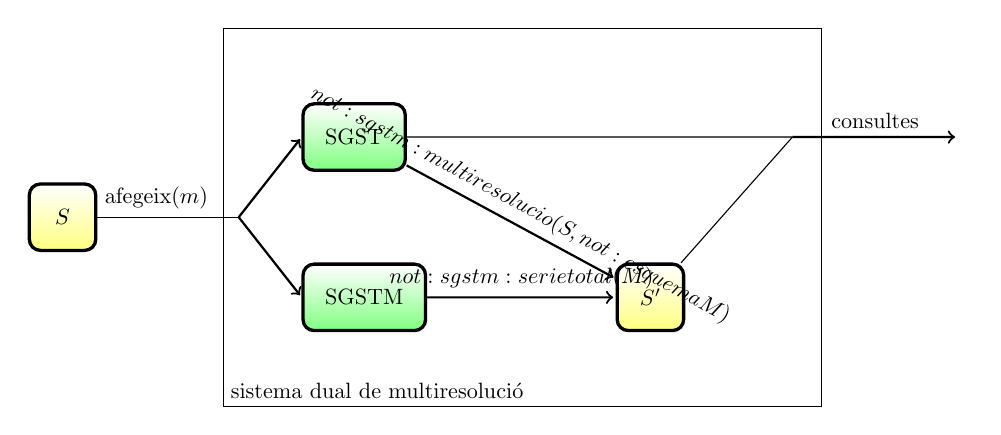
\begin{tikzpicture}[scale=0.8, every node/.style={transform shape}]

      \tikzset{
        mynode/.style={rectangle,rounded corners,draw=black, 
          very thick, inner sep=1em, minimum size=3em, text centered,
          groc},
        myarrow/.style={->, shorten >=1pt, thick},
        mylabel/.style={text width=7em, text centered},
        groc/.style={top color=white, bottom color=yellow!50},
        verd/.style={top color=white, bottom color=green!50},
        roig/.style={top color=white, bottom color=red!50},
      }  






 \node[mynode] (m) {$S$};

 \node[right=2cm of m] (mdins) {};

 \node[mynode, verd, above right=0.6cm and 1cm of mdins] (tsms) {\glstext{SGST}};

 \node[mynode, verd, below right=0.6cm and 1cm of mdins] (mtsms) {\glstext{SGSTM}};

 \node[rectangle,draw,minimum height=6cm,minimum width=9.5cm,right=-0.25cm of mdins] (dual) {};

\draw[shift=( dual.south west)]   
  node[above right] {sistema dual de multiresolució};






 \node[mynode,right=3cm of mtsms] (ts) {$S'$};



 \draw (m.east) -- (mdins.east) node[above right,at start]
 {afegeix$(m)$};

 \draw[myarrow] (mdins.east) -- (tsms.west);
 \draw[myarrow] (mdins.east) -- (mtsms.west);


 \draw[myarrow] (tsms) -- (ts) node[above,midway,sloped]
 {$\glssymbol{not:sgstm:multiresolucio}(S,\glssymbol{not:esquemaM})$}; 
 
 \draw[myarrow] (mtsms) -- (ts) node[above,midway,sloped]
 {$\glssymbol{not:sgstm:serietotal}(M)$};




 \node[right=6cm of tsms] (consdins) {};

 \draw (tsms) -- (consdins.center);
 \draw (ts) -- (consdins.center);

 \node[right=2.5cm of consdins] (consultes) {};
 \draw[myarrow] (consdins.center) -- (consultes) node[above,midway,sloped]
 {consultes};



\end{tikzpicture}



%%% Local Variables:
%%% TeX-master: "../main"
%%% End:

  \caption{Sistema dual \gls{SGST}+\gls{SGSTM}}
  \label{fig:multiresolucio:dual}
\end{figure}

% This may be overcome with dual \acro{DBMS} that share measure input,
% as shown in Figure~\ref{fig:model:mtsms-tsms}. One is a \acro{TSMS}
% for long-term deposit and only consulted in occasional cases, it can
% be \acro{TSMS} with other compression techniques or large size
% \acro{DBMS}. The other is a \acro{MTSMS} that lossy compresses time
% series.

% Then generic queries can be made from \acro{TSMS} information or from
% \acro{MTSMS} selected information, as instance by TotalSeries. In
% Figure~\ref{fig:model:mtsms-tsms} the logical equivalence of applying
% $S'=\totalseries(M)$ to \acro{MTSMS} and $S'=
% \multiresolution(S,\text{sch})$ to \acro{TSMS} is plotted, however the
% implementation consideration are different. If we regard the resulting
% time series $S'$ as a view of database information, then the
% $\multiresolution$ is a view that must be computed fully at every new
% measure addition and $\totalseries$ is a view that can be computed
% incrementally at every new addition as explained next.


% Time series data volume uses to be very big and increases along
% time. However, this increase is due to a continuous acquisition of
% data. When data comes as an ordered sequence of instances it is called
% data stream, then specific \acro{DBMS} are designed to manage data
% stream data \cite{stonebraker05:sigmod}.  \acro{MTSMS} can take
% advantage of data stream orientation in order to simplify the
% consolidation process.  Assuming a time order acquisition of time
% series, the update of a \acro{MTSMS} only consists in the addition of
% new measures and the incremental consolidation of subseries.  As a
% consequence \acro{MTSMS} can be seen as a time series view
% pre-computing system for a pair of aggregation statistics and time
% resolution operations.  Then this pre-computation can be used for
% another queries, limited to the aggregations previously computed, or
% for graphical visualisations like the ones done by RRDtool
% \cite{rrdtool}.

% We then have showed a structure for manipulating in time order as then there are no updates in data and it can be managed more simpler. 

%* Important! dir que si seguim l'addició amb ordre de les mesures, aleshores es pot fer l'stream en els MTSMS ja que no hi ha possibilitat d'operacions d'UPDATE.




\subsection{Conceptes relacionats}


\textcite{marz13:nosql13, marz14:bigdata} generalitzen un concepte
similar al de \gls{SGST} dual, ho emmarquen en l'àmbit dels \gls{SGBD}
per a \emph{Big Data}.  Proposen \gls{SGBD} dissenyats amb tres
nivells, que anomenen arquitectura \emph{Lambda}:
\begin{itemize}
\item Nivell \emph{batch}: Emmagatzema totes les dades originals i
  permet realitzar qualsevol consulta sobre aquestes dades. Preveu que
  algunes consultes operen sobre dades consultades prèviament, per
  tant en aquest nivell es gestionen també aquestes consultes
  precomputades, les quals a més es poden obtenir amb computació
  para\l.lela com per exemple amb Hadoop. Particularment, es considera
  que les dades originals són immutables, és a dir que les bases de
  dades només permeten afegir però no modificar.

\item Nivell \emph{server}: Emmagatzema les consultes precomputades i
  n'ofereix les dades per a altres consultes. Les consultes
  precomputades s'han de tornar a calcular periòdicament i en el
  nivell \emph{server} sempre hi ha la versió calculada més
  recent. Per tant, es preveu que les consultes precomputades no
  ofereixen la informació actualitzada al moment, sinó que hi ha un
  cert temps des que es modifiquen les dades originals fins que té
  impacte en les consultes.

\item Nivell \emph{speed}: Precomputa les mateixes consultes que el
  nivell \emph{batch} però incrementalment, és a dir cada cop que
  s'afegeix una dada nova les dades de la consulta \emph{speed}
  s'actualitzen adequadament.  Aquest nivell només s'usa per a dades
  recents per tal complementar el problema de les dades
  desactualitzades en els nivells \emph{batch} i \emph{server}.
\end{itemize}


Les consultes precomputades d'aquests sistemes semblen una bona
solució per a la computació de les vistes dels \gls{SGBDR}.  Una vista
és un àlies per a una expressió relacional, és a dir una consulta, que
s'utilitza en altres consultes. Per tant, una vista $v$ és una
operació $\text{op1}$ sobre unes $\text{dades}$,
$v:=\text{op1}(\text{dades})$, i s'utilitza una altra consulta
$\text{op2}(v)$ de manera que és equivalent a executar la consulta
$\text{op2}(\text{op1}(\text{dades}))$. Així doncs, el model de vistes
és similar a les consultes que es basen en altres consultes proposat
per \citeauthor{marz14:bigdata} o a les sèries temporals precomputades
que proposem.


En el model relacional \cite[cap.~10. Views]{date04:introduction8} es
considera, conceptualment, que les vistes no s'avaluen quan es
defineixen sinó cada cop que s'executa una consulta que hi opera.  En
les implementacions les vistes poden ser precomputades, aleshores
s'anomenen \emph{snapshots} o \emph{materialized views}, per tal
d'aconseguir un emmagatzematge temporal dels mateixos càlculs per a
diverses consultes. En el context de sistemes de suport a les
decisions, la precomputació també es preveu en el càlcul de taules
resum per a agregacions de les dades \cite[cap.~22. Decision
support]{date04:introduction8}.  Això no obstant, la precomputació de
vistes no sempre comporta una millor eficiència; el concepte de vista
del model permet la substitució algebraica i per tant permet
l'optimització global de la consulta i l'operació continguda a la
vista.


Les vistes precomputades tenen associada una acció per actualitzar de
nou el seu valor. En usar vistes precomputades cal preveure el termini
de validesa dels càlculs precomputats, com ocorre en el nivell
\emph{server} de l'arquitectura \emph{Lambda}. Així doncs, les vistes
precomputades es poden actualitzar de vàries maneres:
\begin{itemize}

\item Es computen periòdicament, com també es proposa en el nivell
  \emph{batch} de l'arquitectura \emph{Lambda}.

\item Es computen cada cop que es modifiquen les dades amb les quals operen, per
  exemple mitjançant operacions de \emph{trigger}. \todo{Els indexos
    als SGBD fan una cosa similar a això?}

\item Quan es modifiquen les dades, s'aplica la mateixa
  operació a la vista precomputada. És a dir, quan es modifiquen les
  dades originals amb una operació $\text{mod}(\text{dades})$ es
  trasllada aquesta operació a la vista $\text{mod}'(\text{dades})$ on
  cal determinar la relació entre $\text{mod}$ i $\text{mod}'$.  És el
  que es proposa en el nivell \emph{speed} de l'arquitectura
  \emph{Lambda} i el que admet el model de \gls{SGSTM} que proposem.
\end{itemize}





% \subsection{Stream orientation}

% \todo{}
% * Dues variacions possibles interessants pels MTSMS:

 
%   - Buffers com a streams, sempre de mida fitada 
%   - Discos enllaçats





%%% Local Variables:
%%% TeX-master: "main"
%%% End:






%  LocalWords:  multiresolució




%------- Annexos ------
\appendix

%------- Glossari ------
\cleardoublepage
%\phantomsection\addcontentsline{toc}{chapter}{\glossaryname}
%\pdfbookmark{\glossaryname}{bookmark:glossari}
\chapter{Nomenclatura i abreviacions}
%\glsaddall
%\printglossary
%%% \printglossary[type=\acronymtype]
\printglossary[type=notation,style=estil-notation]
%------- Bibliografia ------
\cleardoublepage
%\phantomsection\addcontentsline{toc}{chapter}{\bibname}
\pdfbookmark{\bibname}{bookmark:bibliografia}
\printbibliography
%----------------------------------------------

%\backmatter

\end{document}



%%%%%%%%%%%%%%%%%%%%%%%%%%%%%%%%%%%%%%%%%%%%%%%%%%%%%%%%%%%%%%%%%%%%%%%%%%  
% Memòria Tesi Doctoral. Model d'un sistema de gestió multiresolució per a sèries temporals.
%
% Copyright (C) 2011-2013 Aleix Llusà Serra.
% 
% This LaTeX document is free software: you can redistribute it and/or
% modify it under the terms of the GNU General Public License as
% published by the Free Software Foundation, either version 3 of the
% License, or (at your option) any later version.
%
% This document is distributed in the hope that it will be useful, but
% WITHOUT ANY WARRANTY; without even the implied warranty of
% MERCHANTABILITY or FITNESS FOR A PARTICULAR PURPOSE. See the GNU
% General Public License for more details.
%
% You should have received a copy of the GNU General Public License
% along with this document. If not, see <http://www.gnu.org/licenses/>.
%
%
% Aleix Llusà Serra
% Departament de Disseny i Programació de Sistemes Electrònics de la Universitat Politècnica de Catalunya (DiPSE-UPC)
% Escola Politècnica Superior d'Enginyeria de Manresa (EPSEM)
% Av. de les Bases de Manresa, 61-73
% 08242 Manresa (Barcelona)
% PAÏSOS CATALANS 
%
% aleix (a) dipse.upc.edu
% 
% El codi font LaTeX del document es troba a 
% <http://escriny.epsem.upc.edu/projects/rrb/>
%%%%%%%%%%%%%%%%%%%%%%%%%%%%%%%%%%%%%%%%%%%%%%%%%%%%%%%%%%%%%%%%%%%%%%%%%% 